\documentclass[a4paper]{article}

% Packages
\usepackage{graphicx}
\usepackage[margin=1in]{geometry}
\usepackage[utf8]{inputenc}
\usepackage[T1]{fontenc}
\usepackage[backend=bibtex]{biblatex}
\usepackage{comment}
\usepackage{hyperref}
\usepackage{amsmath}

\usepackage{CJKutf8}


\addbibresource{references.bib}

\title{Evaluation of Pre-Trained Models for Many-to-English Translation}
\author{Stefan Liemawan Adji}
\date{\today}

\begin{document}

\maketitle


\begin{abstract}
    Machine translation (MT) has become an essential tool for overcoming language barriers in an increasingly globalised world. Today, there are pre-trained models (PTMs) specifically designed for automatic machine translation. This paper evaluates the performance of various pre-trained models (PTMs) for many-to-English translation. The models assessed include OPUS-MT \cite{tiedemann-2020-opus-mt}, mBART-50 \cite{liu-2020-mbart}, NLLB-200 \cite{nllb200-2020}, and M2M-100 \cite{fan-2020-m2m100}. Using a dataset curated from the Tatoeba repository, comprising 1,323 parallel sentence pairs across 14 source languages, translation quality is measured using BLEU, SacreBLEU, and METEOR scores. The results indicate that OPUS-MT, a one-to-one PTM, outperforms multilingual models in one-to-English translation tasks, with mBART-50 leading among the multilingual PTMs. These findings highlight the strengths and limitations of both specific language and multilingual PTMs in machine translation.
\end{abstract}

\section{Introduction}

According to Ethnologue \cite{ethnologue-2024}, 7,164 languages currently exist and in use today, with 40\% of them considered endangered. As of July 2024, 243 languages are supported by Google Translate (according to Wikipedia \cite{wikipedia-google-translate}). In modern times, the need for translation services has surged due to the growing exchange of information across different regions that speak various languages \cite{okpor-2014-machine-ta}.

Machine translation (MT) is the task of automatically translating from one language to another. This can be done through text or audio. It can be traced back to 1949 \cite{weaver-1999}, with the first public demonstration of an MT system on January 7, 1954, in collaboration with IBM, where 49 Russian sentences were translated into English using a limited vocabulary of 250 words and 6 grammar rules \cite{hutchins-2006-first-mt}. However, over the next several decades, growth were limited for machine translation, with 1956-1966 considered the decade of high expectation and disillusion, and 1967-1976 dubbed 'the quiet decade' \cite{hutchins-2001-mt-50-years}. Then in 1989, the dominance of the rule-based approach has been challenged by the rise of new methods and strategies, collectively referred to as ‘corpus-based’ methods (data-driven) \cite{hutchins-1994-research-methods-mt,hutchins-1998-development-mt}. Subsequently, statistics-based approaches for MT re-emerged, bolstered by the recent success of probabilistic techniques in speech recognition. Statistical machine translation \cite{lopez-2008-smt} dominated the domain between late 1990s through the early 2010s, before largely being surpassed by neural machine translation (NMT) \cite{cho-2014-properties,sutskever-2014-seq2seq}.

Since the introduction of Transformers in 2017 \cite{vaswani-2017-attention}, Natural Language Processing (NLP) and machine translation in particular reached a giant milestone. The following years saw the birth of Large Language Models (LLMs) such as BERT \cite{devlin-2019-bert}, GPT \cite{openai-2024-gpt4}, and T5 \cite{raffel-2023-t5}, which revolutionised both MT and the whole field of NLP. Then in early 2020s, several pre-trained models (PTM) that are specifically designed for machine translation emerged, OPUS-MT \cite{tiedemann-2020-opus-mt} produced numerous PTMs designed for one-to-one translations. Additionally, multilingual models: mBART-50 \cite{liu-2020-mbart}, NLLB-200 \cite{nllb200-2020}, and M2M-100 \cite{fan-2020-m2m100} have also been published, growing popularity as multilinguality has been shown to allow for sharing information among languages \cite{garcia-2020-multilingual}. Most of these models are trained on diverse set of languages, allowing for many-to-many translation: able to translate between any of the supported pair of languages. This allows the models to generalise over shared lexical and linguistic among languages, and have been shown to increase performance compared to one-to-one translation models \cite{liu-2020-mbart}.

Despite these advancements, pre-trained models are often evaluated using different set of benchmarks \cite{liu-2020-mbart,nllb200-2020,fan-2020-m2m100,wei-2023-polylm}, making it difficult to gauge their relative effectiveness across various languages. Nevertheless, there does not seem to be much work on comparing or benchmarking different pre-trained models in machine translation. Intento published 'The State of Machine Translation 2024' \cite{intento-2020} providing an in-depth evaluation of popular MT engines and LLMs. However, the biggest drawback in this report is that the selected LLMs are general LLMs such as GPT, LLaMa, Mistral, instead of MT-specific LLMs.

Through simple experimentations, this paper aims to evaluate the performance of existing pre-trained models (PTMs) on many-to-English translation across 14 source languages. Although fine-tuning multilingual PTMs has been proven to increase model performance \cite{cooper-stickland-2021-recipes}, no pre-training or fine-tuning is performed in this study for simplicity reasons. A dataset is curated from the Tatoeba repository \cite{tatoeba}, containing 1,323 parallel sentence pairs across source and target languages. The models include a one-to-one PTMs: OPUS-MT \cite{tiedemann-2023-democratizing,tiedemann-2020-opus-mt}, and multilingual PTMs: such as mBART-50 \cite{liu-2020-mbart}, NLLB-200 \cite{nllb200-2020}, and M2M-100 \cite{fan-2020-m2m100}. The performance of these models is evaluated using the BLEU \cite{papieni-2002-bleu}, SacreBLEU \cite{post-2018-sacrebleu}, and METEOR \cite{lavie-2007-meteor}.

The result indicates that OPUS-MT outperforms all other multilingual models in one-to-English translation, highlighting the superiority of specific languages PTMs compared to multilingual PTMs. mBART-50 shows the best performance among other multilingual PTMs: M2M-100 and NLLB-200.

\section{Literature Review}

\subsection{Pre-Trained Models for Machine Translation}

The encoder-decoder approach \cite{cho-2014-properties} remains as the foundation architecture for many sequence-to-sequence models in machine translation. Attention mechanism has been used for Neural Machine Translation (NMT) \cite{bahdanau-2016-nmt-jointly, luong-2015-effective-attention} before the release of the transformer \cite{vaswani-2017-attention}

Currently, Pre-Trained-Models (PTMs) have become a cornerstone in machine translation, leveraging large datasets and powerful architectures to achieve state-of-the-art performance \cite{han-2021-ptms}. Most PTMs support two kinds of translations: one-to-one translation and many-to-many translation (multilingual models).

One-to-One Translation refers to a translation approach where a model is specifically trained to translate between one source language and one target language. This setup is characterised by having a dedicated model for each unique language pair. OPUS-MT \cite{tiedemann-2020-opus-mt} and Facebook Fairseq \cite{ott-2019-fairseq} are examples of PTMs that support one-to-one translation. Multilingual models have also gained significant prominence, enabling many-to-many translation, where a single model can translate between multiple source and target languages \cite{aharoni-2019-massively-multilingual}.

OPUS-MT \cite{tiedemann-2020-opus-mt} is a project dedicated to creating and providing free resources for machine translation,providing over a thousand of PTMs of direct one-to-one translations. In contrast, mBART \cite{liu-2020-mbart}, M2M \cite{fan-2020-m2m100}, NLLB-200 \cite{nllb200-2020}, are massively multilingual models that support many-to-many translation language.

\subsection{Parallel Corpora}

Corpora are large and structured sets of texts used for linguistic research and analysis. Thus, parallel corpora are defined as sets of texts in a given source language along with their translations in another target language \cite{lefer-2020-parallel-corpora}. It can be bilingual or multilingual, and are crucial for training and evaluating machine translation. Languages without or with limited parallel corpora are referred as \textbf{low-resources language}.

Since the early 2000s, English has often been used as an intermediary language, meaning texts originally written in languages are first translated into English, and then from English into other languages, resulting in most target texts being translations of translations \cite{lefer-2020-parallel-corpora}. This is called indirect translation, and posed for many problems in translations as terms can be ambiguous with varying or similar meanings \cite{rosa-2017-indirect-translation-problems}.

Neural Machine Translation (NMT) systems require vast amounts of training data, and thus the availability of parallel corpora is crucial for building effective models \cite{koehn-2017-challenges}. The lack of extensive parallel corpora, especially for low-resource languages, leads to suboptimal performance in NMT techniques compared to their high-resource counterparts \cite{ranathunga-2023-nmt-low-res}. OPUS \cite{opus} is a comprehensive collection of open-source parallel corpora used extensively in the field of machine translation (MT). It includes corpora for 744 languages and contains over 1,210 different datasets, amassing a total of 45,945,946,108 sentence pairs. Tatoeba \cite{tatoeba} is another prominent resource in the field of MT and NLP, known for its extensive collection of translated sentences. As of July 2024, it contains 12,186,207 sentences over 423 supported languages, growing daily through volunteer contributions.

Several datasets are often used for evaluation in machine translation. The Tatoeba Challenge \cite{tiedemann-2020-tatoeba-challenge} covers 487 languages in 4,024 language pairs, including 657 test sets sourced from Tatoeba website, covering 138 languages. The TED Talks dataset \cite{ye-2018-word-embeddings-ted} contains transcripts from TED talks for more than 50 languages. IWSLT \cite{agarwal-iwstl-2023} also contains TED talks data, but paired with English translations. Finally, WMT \cite{barrault-2020-wmt} is an annual event that organises tasks for machine translation and provides a collection of datasets for benchmarking and evaluating translation systems.

While these datasets can be used to evaluate translation performance between any language pairs, they do not contain parallel corpora between different languages. Corpus between English and French for example, contains different text to the corpus between English and Spanish. Therefore, they do not support easy evaluation for many-to-English translations. Furthermore, papers often use different datasets and versions to evaluate their model performance, making direct comparison challenging.

mBart \cite{liu-2020-mbart} uses WMT19 for English-German translation and TED15 for Chinese-English translation. M2M-100 \cite{fan-2020-m2m100} uses 7 different datasets shared across languages. NLLB-200  \cite{nllb200-2020} uses FLORES dataset, designed for low-resources languages. OPUS-MT \cite{tiedemann-2023-democratizing,tiedemann-2020-opus-mt} models use datasets from Tatoeba challenges.


\section{Methodology}

\subsection{Dataset}

Tatoeba is a vast, continuously expanding database consisting sentences and their translations, built through the contributions of thousands of volunteers, offering a tool that allows users to see examples of how words are used in sentences \cite{tatoeba}. They currently have 12,132,349 sentences and 423 supported languages, with around one to two thousand new sentences added daily, on average. The English sentence dataset contains 1,905,089 sentences, the largest one in their repository, with Russian in the second place with 1,066,633 sentences. Some languages supported on the website is shown in Figure \ref{fig:tatoeba_languages} and Figure \ref{fig:tatoeba_top_bottom_languages}, sorted from the biggest corpus.

\begin{figure}[htbp]
    \centering
    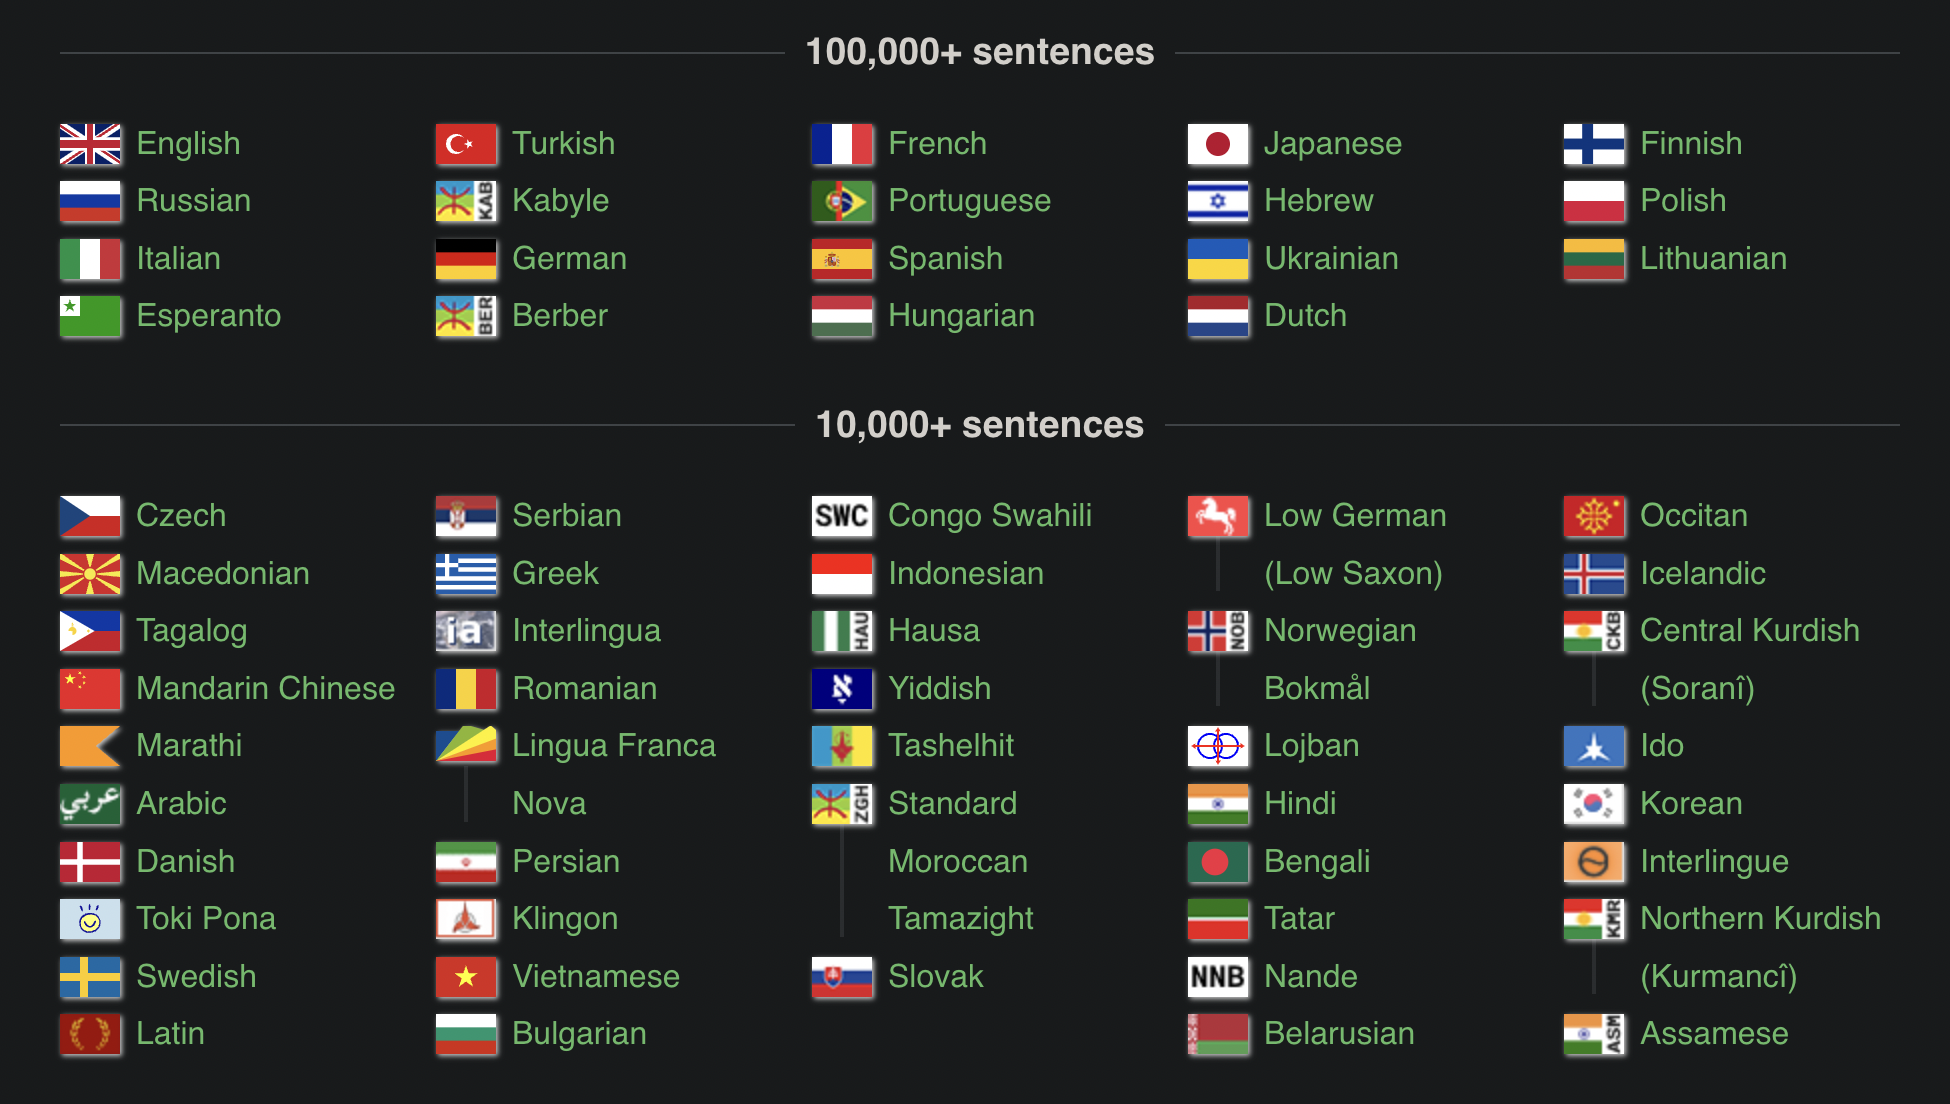
\includegraphics[width=0.9\linewidth]{images/tatoeba_languages.png}
    \caption{Tatoeba's languages repository with 10,000+ sentences and 100,000+ sentences \cite{tatoeba}}
    \label{fig:tatoeba_languages}
\end{figure}


\begin{figure}[htbp]
    \centering
    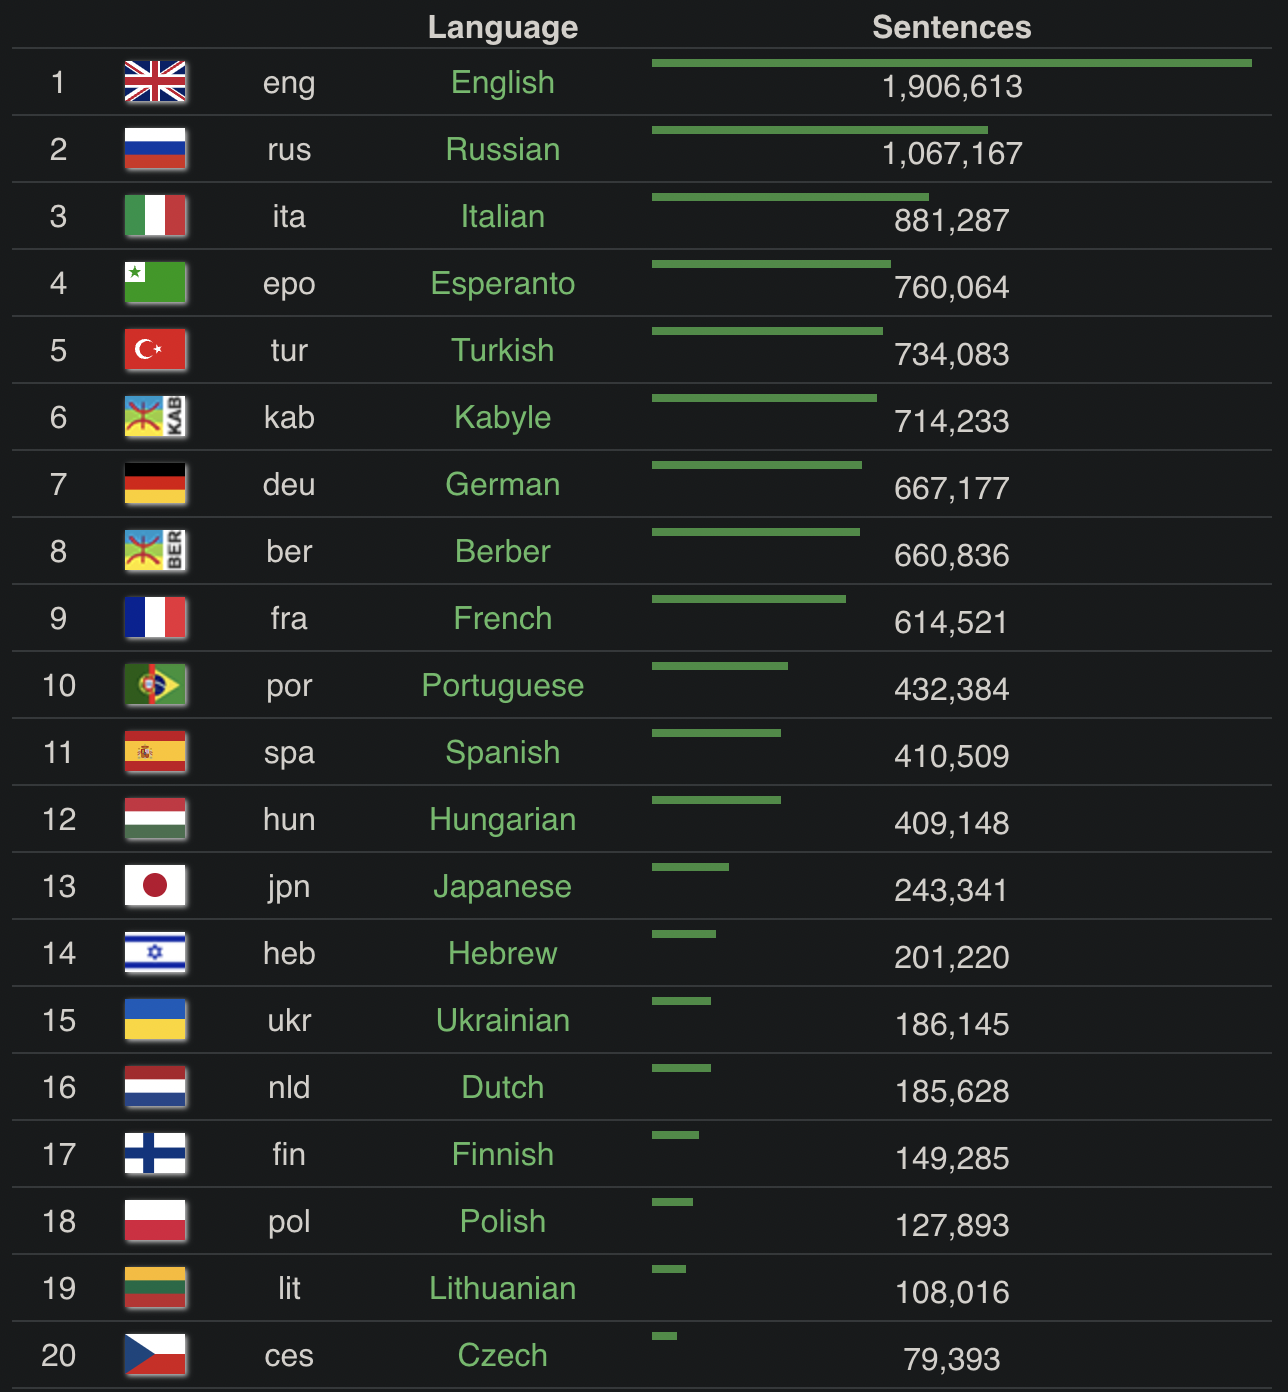
\includegraphics[width=0.5\linewidth]{images/tatoeba_top_20_lang.png}
    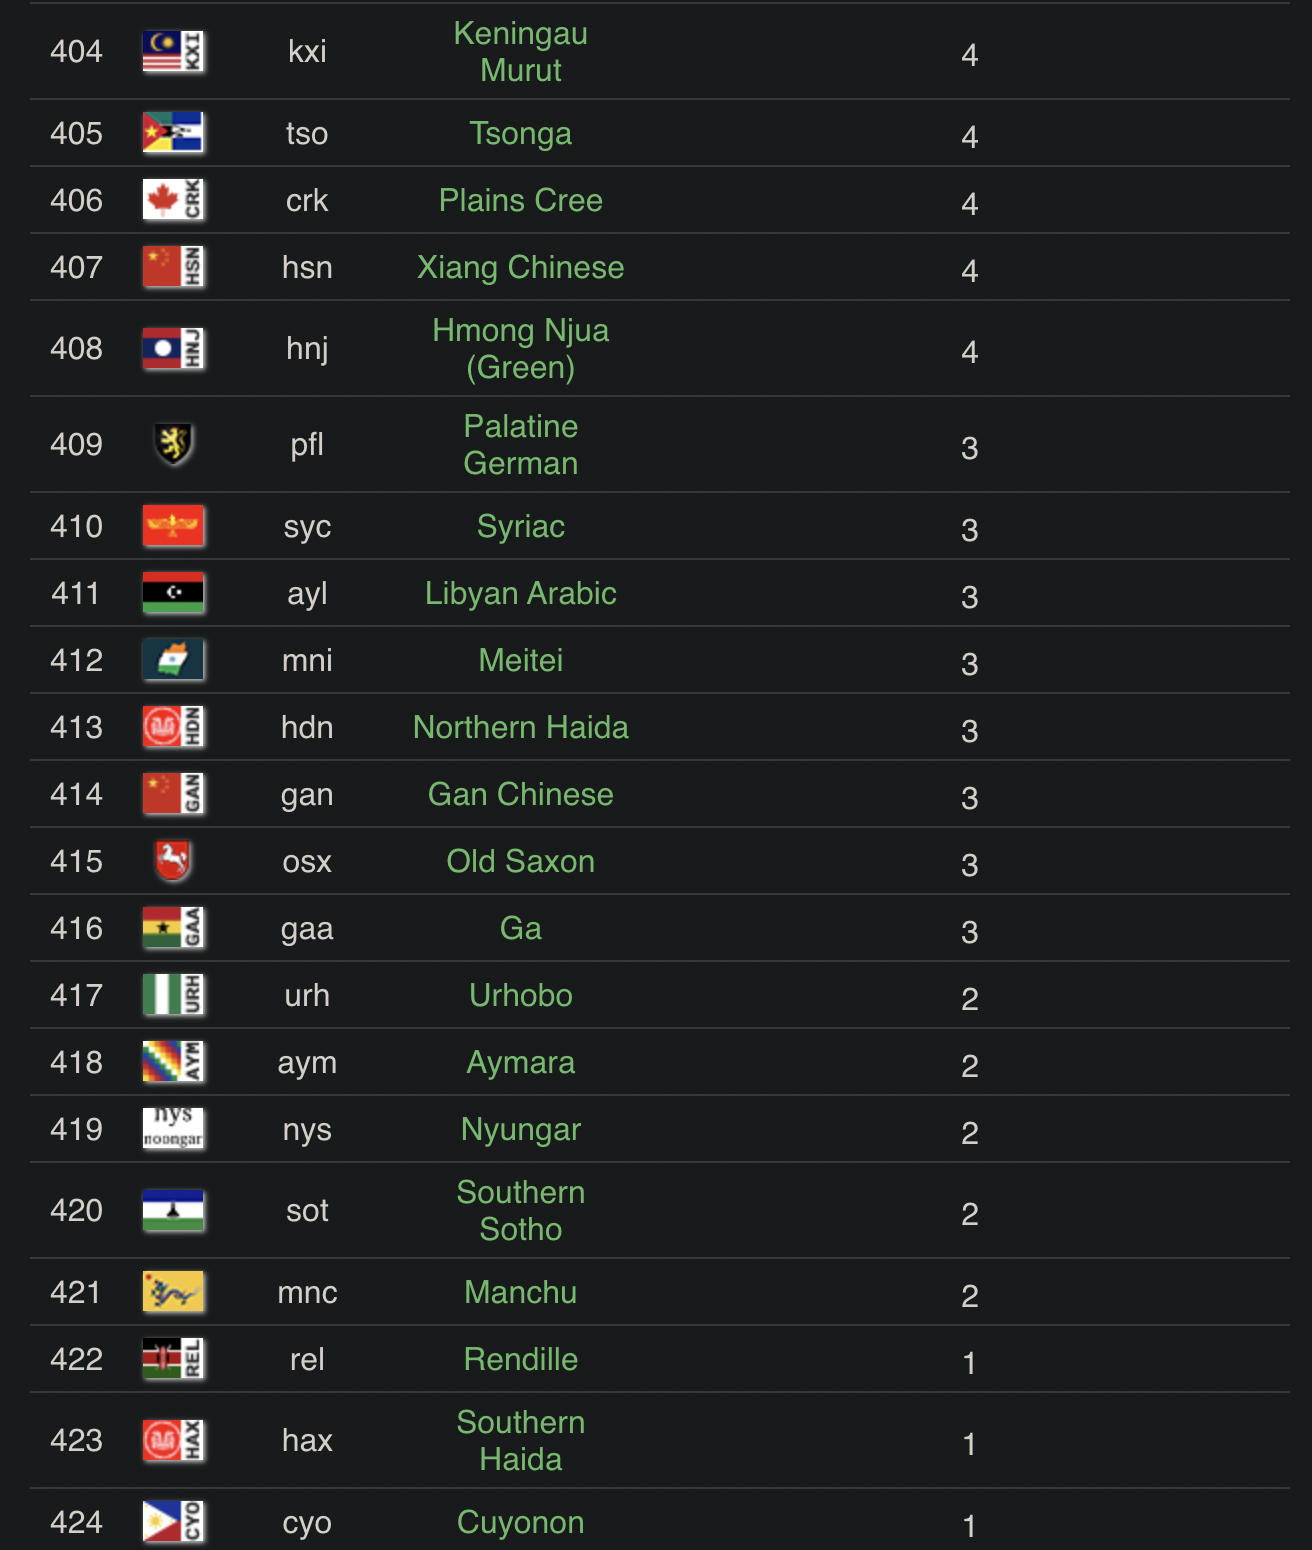
\includegraphics[width=0.46\linewidth]{images/tatoeba_bottom_20_lang.png}
    \caption{Tatoeba top 20 and bottom 20 languages based on sentences count \cite{tatoeba}}
    \label{fig:tatoeba_top_bottom_languages}
\end{figure}


\begin{table}[htbp]
    \centering
    \begin{tabular}{|l|l|r|}
        \hline
        \textbf{No.} & \textbf{Language} & \textbf{Sentence Pairs Count} \\
        \hline
        1            & Chinese           & 68,814                        \\
        2            & Dutch             & 155,856                       \\
        3            & Finnish           & 102,202                       \\
        4            & French            & 405,088                       \\
        5            & German            & 501,145                       \\
        6            & Hebrew            & 172,082                       \\
        7            & Hungarian         & 171,698                       \\
        8            & Italian           & 624,160                       \\
        9            & Japanese          & 270,116                       \\
        10           & Polish            & 77,345                        \\
        11           & Russian           & 722,837                       \\
        12           & Spanish           & 265,253                       \\
        13           & Turkish           & 710,279                       \\
        14           & Ukrainian         & 214,244                       \\
        \hline
    \end{tabular}
    \caption{List of chosen languages for evaluation}
    \label{table:eval_languages}
\end{table}

Table \ref{table:eval_languages} show the 14 languages selected for this project. Languages are chosen based on its resources' availability in Tatoeba, as well as considering supported languages in most PTMs models. Thus, the languages chosen here can be considered as moderate to high resources languages.

To build the dataset, sentences in English are first downloaded, containing 1,898,494 sentences (it is unclear why it is less than the number stated in the Tatoeba website). Then for each language, sentence pairs between English and source languages are downloaded individually and compiled. The result is a single Dataframe containing 1,323 parallel sentences in all 14 languages, this will be treated as a test set to evaluate the models performance on each language. Note that in the case of multiple reference translations are available for the same sentence in English, only the first sentence is taken while the rest is discarded. Therefore, there is only one reference for each candidate sentence.

Sentences typically consist of everyday phrases such as 'I have to go to sleep', 'That is intriguing', and 'Where do you live?'. They may also include single-word exclamations like 'Speak!', 'So what?', or 'Look!'. Additionally, multiple sentences such as 'You may write in any language you want. On Tatoeba, all languages are considered equal', and 'Guns don't kill people. People kill people' can be found inside the corpus. A few of them also include human names, 'Compare your answer with Tom's', 'Muiriel is 20 now'. All of the sentences are straightforward and literal, without the use of linguistic features such as metaphors or sarcasm. Therefore, machine translation process should be straightforward on this level. Figure \ref{table:parallel_sentence} shows two examples of parallel sentences in the final dataset, across all 14 languages and the original English sentence.


\begin{CJK}{UTF8}{gbsn}
    \begin{table}[htbp]
        \centering
        \begin{tabular}{|l|l|l|}
            \hline
            \textbf{Language} & \textbf{Sentence 1}                   & \textbf{Sentence 2}                   \\
            \hline
            English           & I have to go to sleep.                & So what?                              \\
            Chinese           & 我该去睡觉了。                               & 那又怎樣?                                 \\
            Dutch             & Ik moet gaan slapen.                  & Dus?                                  \\
            Finnish           & Minun täytyy mennä nukkumaan.         & Mitä sitten?                          \\
            French            & Je dois aller dormir.                 & Et alors ?                            \\
            German            & Ich muss jetzt schlafen.              & Na und?                               \\
            Hebrew            & <hidden-due-to-latex-incompatibility> & <hidden-due-to-latex-incompatibility> \\
            Hungarian         & Aludni kell mennem.                   & És akkor mi van?                      \\
            Italian           & Devo andare a dormire.                & E allora?                             \\
            Japanese          & 私は眠らなければなりませ                          & だから何?                                 \\
            Polish            & Muszę iść spać.                       & No i co?                              \\
            Russian           & Мне пора идти                         & Так что?                              \\
            Spanish           & Tengo que irme a dormir.              & ¿Entonces qué?                        \\
            Turkish           & Yatmaya gitmek zorundayım.            & Öyleyse ne yapmalı?                   \\
            Ukrainian         & Маю піти спати.                       & Ну то що?                             \\
            \hline
        \end{tabular}
        \caption{A snippet of the dataset}
        \label{table:parallel_sentence}
    \end{table}
\end{CJK}


\begin{figure}[htbp]
    \centering
    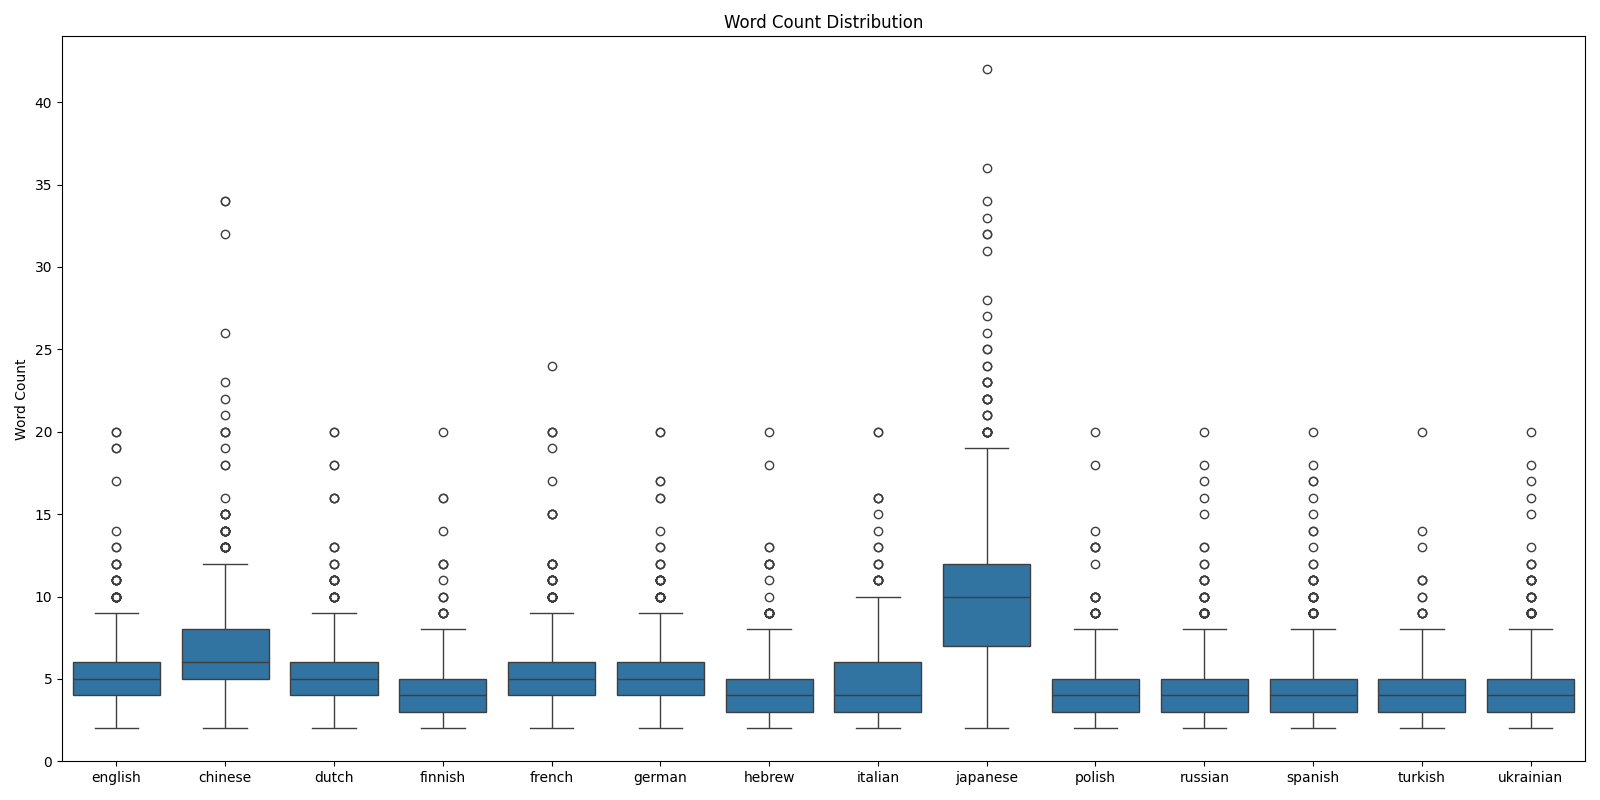
\includegraphics[width=1\linewidth]{figures/word_count_box.png}
    \caption{Dataset word count distribution per language, Chinese and Japanese sentences are counted per letter.}
    \label{fig:word_count_box}
\end{figure}

Figure \ref{fig:word_count_box} shows a box plot of sentences word count. The median for Dutch, Finnish, French, German, Hebrew, Italian, Polish, Russian, Spanish, Turkish, Ukrainian seems relatively low, with a moderate spread. A few to moderate count of outlier exist in all languages, suggesting occasional longer sentences, with the highest variability seen in Japanese. Note that for Chinese and Japanese the count is based on each Chinese/Japanese letter, which explains their higher interquartile range (IQR) and larger numbers of outliers.

\subsection{Proposed Pre-Trained Models}

\subsubsection{OPUS-MT}

\textbf{OPUS-MT} \cite{tiedemann-2023-democratizing,tiedemann-2020-opus-mt} provides over 1,000 pre-trained models for translation between numerous language pairs. The architecture is based on MARIAN-NMT \cite{mariannmt}, based on a standard transformer setup: 6 self-attentive layers in both the encoder and decoder networks, each with 8 attention heads per layer \cite{tiedemann-2020-opus-mt}. While OPUS-MT support both monolingual and multilingual PTMs, the multilingual models seem to lack proper documentation and therefore excluded from this experiment.

\subsubsection{mBART-50}

\textbf{mBART} \cite{liu-2020-mbart} is a sequence-to-sequence denoising auto-encoder model specifically designed for multilingual tasks. The mBART-50 variant supports many-to-many translations for over 50 languages.

\begin{figure}[htbp]
    \centering
    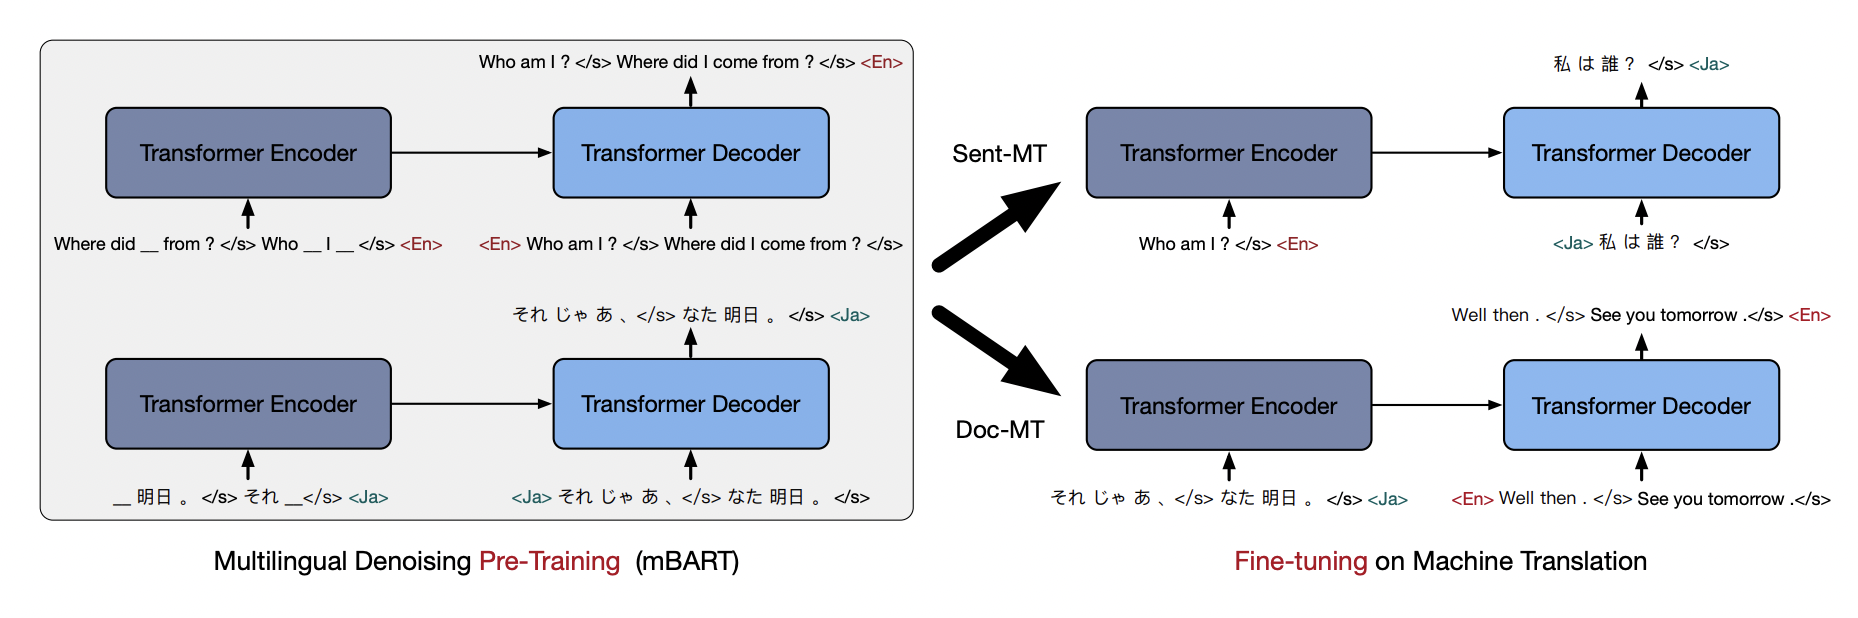
\includegraphics[width=0.9\linewidth]{images/mbart.png}
    \caption{mBART framework for Multilingual Denoising Pre-training (left) and fine-tuning on downstream MT tasks
        (right) \cite{liu-2020-mbart}}
    \label{fig:mbart}
\end{figure}

Figure \ref{fig:mbart} shows the architecture of mBART's key features multilingual denoising pre-training and fine-tuning. It is shown that the model achieved consistent performance gains through pre-training in low-to-medium resource sentence level MT \cite{liu-2020-mbart}. The "denoising" here refers to a pre-training technique used to improve the model's ability to generate coherent and accurate translations by training it to reconstruct original sentences from corrupted (noisy) versions.

\subsubsection{M2M-100}

\textbf{M2M-100} \cite{fan-2020-m2m100} is designed to perform direct translation between 100 languages without relying on English as an intermediate language.


\begin{figure}[htbp]
    \centering
    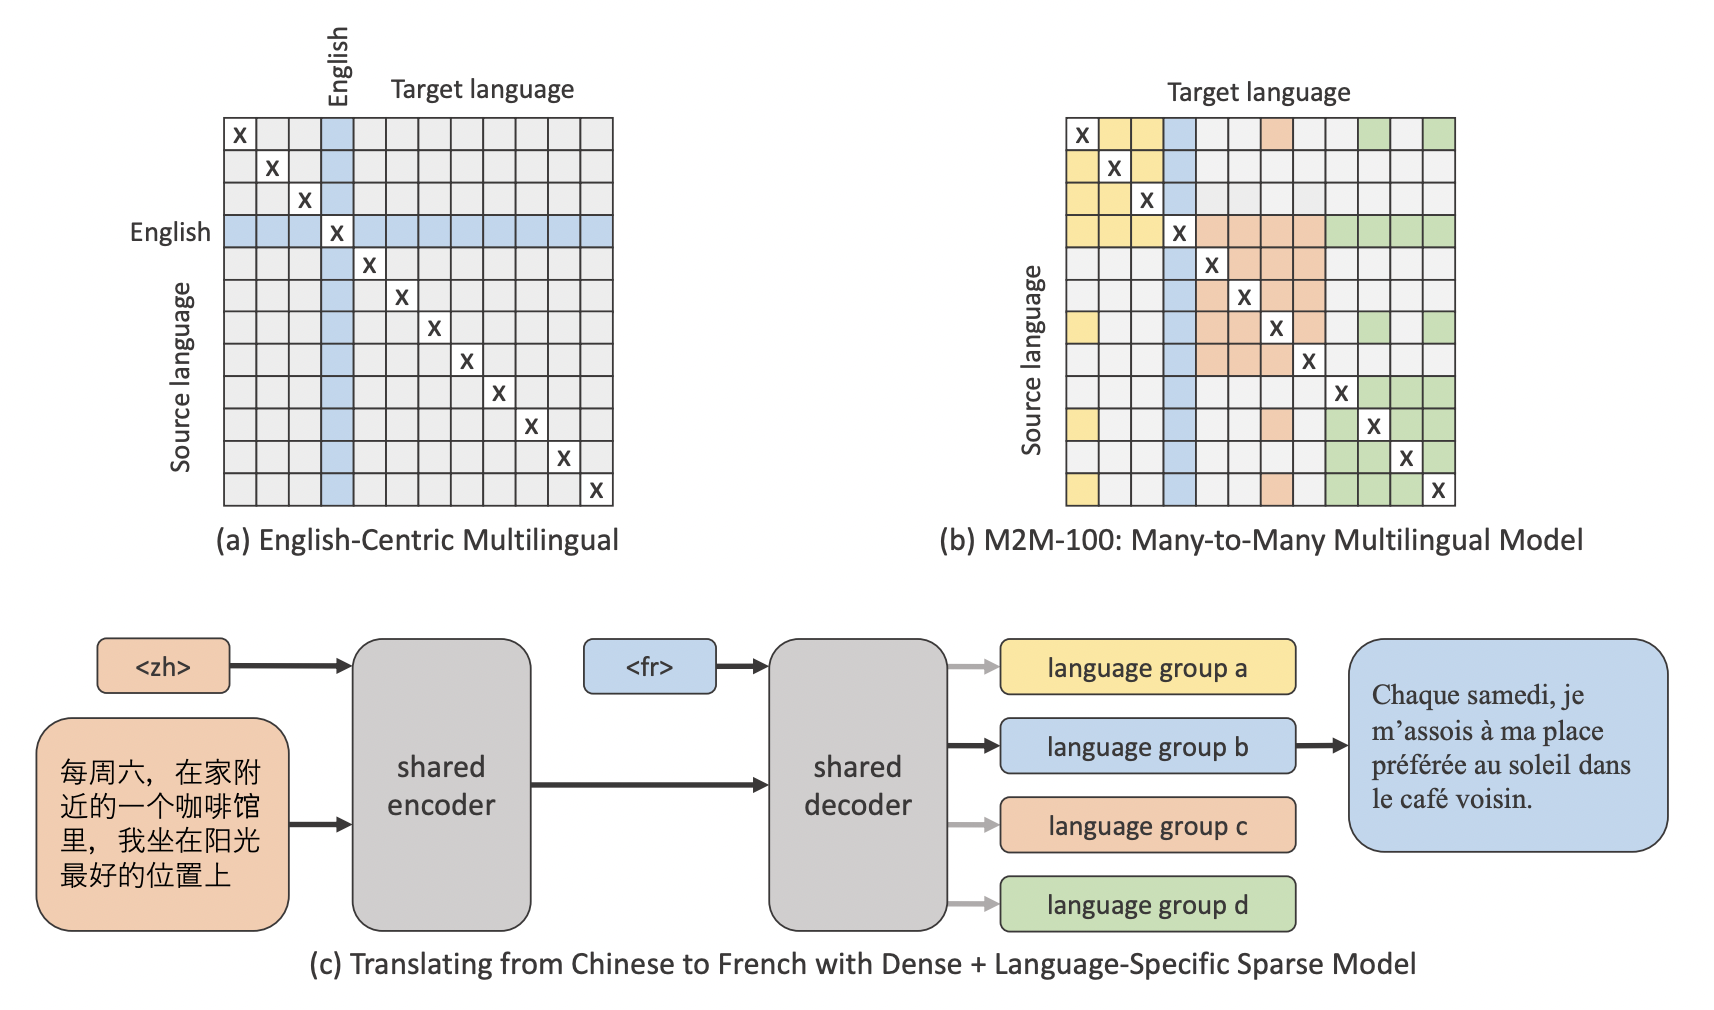
\includegraphics[width=0.9\linewidth]{images/m2m.png}
    \caption{Summary of M2M dataset and multilingual model.}
    \label{fig:m2m}
\end{figure}

Figure \ref{fig:m2m} show the inner working of the M2M model. The English-centric dataset (top left) includes training data exclusively involving translations to and from English, while the many-to-many multilingual setting (top right) involves direct translation data among multiple language pairs \cite{fan-2020-m2m100}. The M2M-100 model then integrates dense and sparse language-specific parameters to enable direct translation between languages (bottom part of Figure \ref{fig:m2m}).

\subsubsection{NLLB-200}

\textbf{NLLB-200} \cite{nllb200-2020} is built to handle translation tasks across a broad spectrum of languages, including many that are low-resource or underrepresented in existing datasets. It supports translations for 200 languages, including numerous underrepresented languages, and is currently one of the most extensive multilingual machine translation models. The model employs a Mixture of Experts (MoE) architecture and achieves state-of-the-art (SoTA) results across many language pairs, even surpassing Meta's previous model, M2M-100 \cite{nllb200-2020}.


\begin{figure}[htbp]
    \centering
    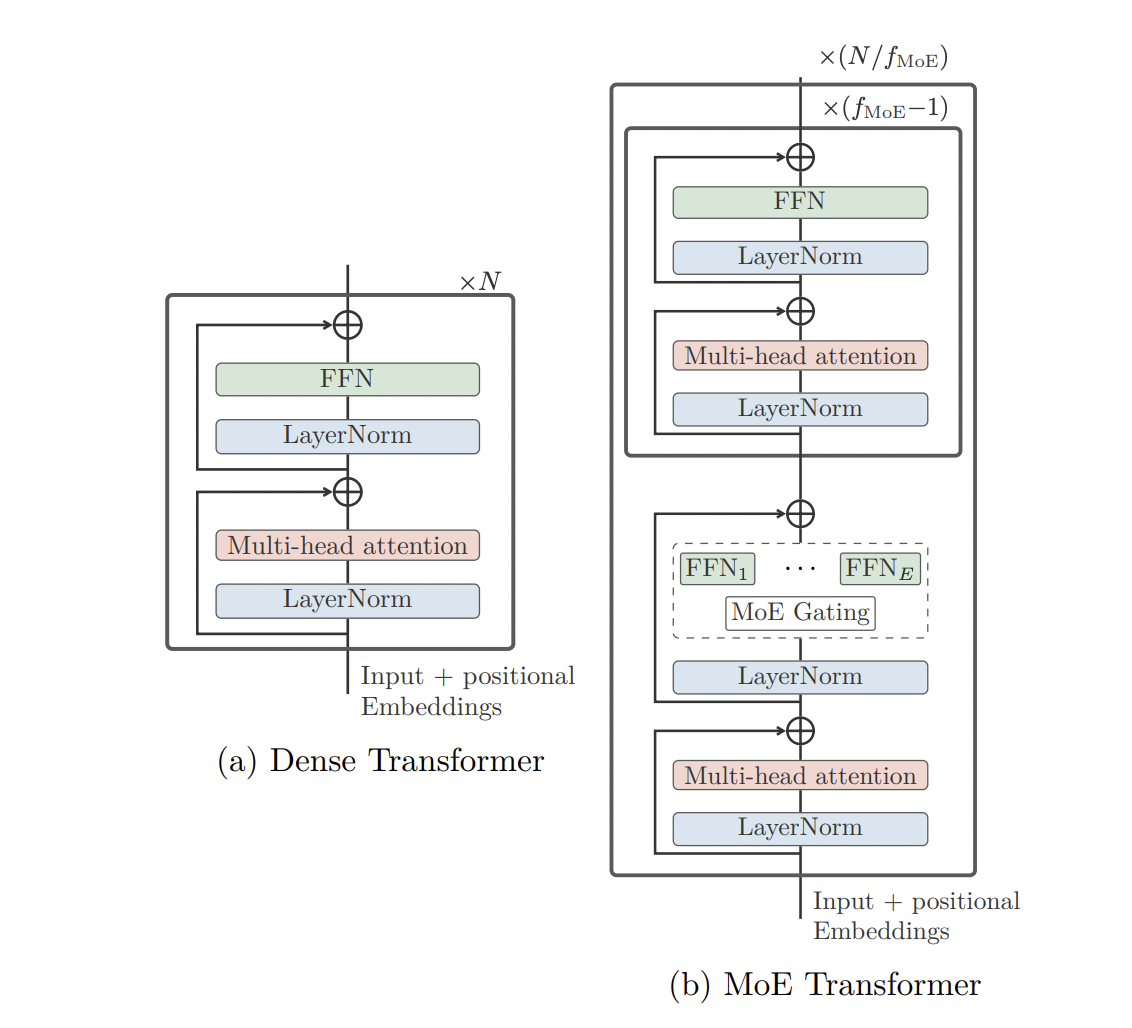
\includegraphics[width=0.7\linewidth]{images/nllb.png}
    \caption{NLLB pipeline \cite{nllb200-2020}}
    \label{fig:nllb}
\end{figure}

Figure \ref{fig:nllb} shows the Dense Transformer and MoE Transformer layers implemented within the model. MoE \cite{masoudnia-2012-moe} utilises a gating mechanism to route different inputs to different subsets of experts (sub-networks), allowing the model to handle various linguistic phenomena efficiently. Additionally, the model is then trained on a diverse set of languages, complemented with back-translation and data augmentation to generate additional data for low-resource languages \cite{nllb200-2020}.

% The original paper is 192 pages long and impossible to be dissected in just one section.


\subsection{Evaluation Metrics}


In this project, a variant of BLEU \cite{papieni-2002-bleu} called SacreBLEU \cite{post-2018-sacrebleu} and METEOR \cite{lavie-2007-meteor} will be used in this experiment due to their popularity, simplicity, and ease-of-use.

While other metrics such as Crosslingual Optimized Metric for Evaluation of Translation (COMET) \cite{rei-2020-comet} and BERTSCore \cite{zhang-2020-bertscore} exist, they involve using a deep neural network or a transformer to evaluate, which naturally increase computational cost and slow down calculation greatly.

\subsubsection{BLEU}

Bilingual Evaluation Understudy (BLEU) \cite{papieni-2002-bleu} is the most commonly used metrics for machine translation (MT). It assesses how well a candidate translation matches the reference translation using precision metrics for n-grams and incorporates a brevity penalty to prevent overly short translations from achieving high scores.

The n-gram precision, as presented in the original BLEU paper \cite{papieni-2002-bleu}, is calculated as:

\begin{equation}
    p_n = \frac{\sum_{C \in \{Candidates\}} \sum_{\text{n-gram} \in C} \text{Count}_{\text{clip}}(\text{n-gram})}{\sum_{C \in \{Candidates\}} \sum_{\text{n-gram} \in C} \text{Count}(\text{n-gram})}
\end{equation}

Where:
\begin{itemize}
    \item \( p_n \) is the precision for n-grams.
    \item \( \sum_{C \in \{Candidates\}} \) denotes the summation over all candidate translations.
    \item \( \sum_{\text{n-gram} \in C} \) denotes the summation over all n-grams in a candidate translation \( C \).
    \item \( \text{Count}_{\text{clip}}(\text{n-gram}) \) is the clipped count of the n-gram, which is the count of the n-gram in the candidate translation limited by the maximum count of that n-gram in any reference translation.
    \item \( \text{Count}(\text{n-gram}) \) is the count of the n-gram in the candidate translation.
\end{itemize}

Thus, the BLEU score is calculated as:

\begin{equation}
    \text{BLEU} = BP \cdot \exp \left( \sum_{n=1}^{N} w_n \log p_n \right)
\end{equation}

Where:
\begin{itemize}
    \item \( BP \) is the brevity penalty.
    \item \( p_n \) is the precision for n-grams.
    \item \( w_n \) is the weight for each n-gram (often uniformly distributed, so \( w_n = \frac{1}{N} \)).
\end{itemize}

The brevity penalty (BP) is calculated as:

\begin{equation}
    BP = \begin{cases}
        1                     & \text{if } c > r    \\
        e^{(1 - \frac{r}{c})} & \text{if } c \leq r
    \end{cases}
\end{equation}

Where:
\begin{itemize}
    \item \( c \) is the length of the candidate translation.
    \item \( r \) is the effective reference length.
\end{itemize}

The machine translation community's rely heavily BLEU score, however, it has several drawbacks. The metric has been reported to not correlate strongly with human judgement, showing variations in translation that could mean that a higher BLEU score does not necessarily indicate a true enhancement in translation quality \cite{callison-burch-2006-reevaluating-bleu}.

Furthermore, It is challenging to directly compare BLEU scores between paper \cite{post-2018-sacrebleu}. Thus, the author proposed a standardised variant called SacreBLEU \cite{post-2018-sacrebleu}, designed to ensure easy, consistent, and comparable evaluation across different implementations and research studies.

\subsubsection{METEOR}

Metric for Evaluation of Translation with Explicit ORdering (METEOR) \cite{lavie-2007-meteor} assesses a translation by calculating a score that reflects explicit word-to-word matches between the reference and a candidate translation \cite{agarwal-2008-meteor-mbleu-mter}. It is designed to address some limitations of the BLEU score, allowing matches between simple morphological variants and synonyms.

\begin{equation}
    \text{METEOR} = (1 - \gamma \cdot \text{frag}) \cdot \frac{P \cdot R}{\alpha \cdot P + (1 - \alpha) \cdot R}
\end{equation}

Where:
\begin{itemize}
    \item \(P\) is the precision,
    \item \(R\) is the recall,
    \item \(\text{frag}\) is the fragmentation penalty,
    \item \(\gamma\) is a parameter that controls the weight of the fragmentation penalty, commonly 0.5,
    \item \(\alpha\) is a parameter that controls the balance between precision and recall, commonly 0.9,
\end{itemize}

\subsection{Inference Details}

OPUS-MT models are taken from the Helsinki-NLP repository. The 'mbart-large-50-many-to-many-mmt' is used, 'm2m100\_418M', and 'nllb-200-distilled-600M'. All models are taken using the transformers \cite{wolf-etal-2020-transformers} library from Hugging Face \cite{huggingface}. Batch size of 4 is used in all models. Translations are first generated and saved into CSV files, before calculating the metrics score.

The sacrebleu packages from pip is used to calculate SacreBLEU \cite{post-2018-sacrebleu}. For BLEU and METEOR, the NLTK \cite{bird-2009-natural} package is used. Corpus BLEU is implemented for both SacreBLEU and BLEU in the calculations.
\section{Evaluation}


\begin{table}[htbp]
    \centering
    \begin{minipage}{0.49\linewidth}
        \footnotesize
        \begin{tabular}{|l|r|r|r|}
            \hline
            \textbf{Language} & \textbf{BLEU}   & \textbf{SacreBLEU} & \textbf{METEOR} \\
            \hline
            Chinese           & 0.0971          & \textit{59.5098}   & 0.7953          \\
            Dutch             & 0.0974          & 69.8803            & 0.8471          \\
            Finnish           & 0.0965          & 66.6267            & 0.8296          \\
            French            & 0.0967          & 69.8185            & 0.8357          \\
            German            & 0.0969          & 69.7422            & 0.8419          \\
            Hebrew            & 0.0977          & 66.5149            & 0.8229          \\
            Italian           & 0.0979          & 74.1298            & 0.8584          \\
            Japanese          & 0.0960          & 63.1435            & \textit{0.7893} \\
            Polish            & \textit{0.0952} & 61.9026            & 0.8425          \\
            Russian           & 0.0974          & 66.7046            & 0.8179          \\
            Spanish           & 0.0979          & 71.4174            & 0.8463          \\
            Turkish           & \textbf{0.0980} & 72.6551            & 0.8460          \\
            Ukrainian         & 0.0978          & \textbf{75.4447}   & \textbf{0.8667} \\
            \hline
        \end{tabular}
        \caption{OPUS-MT result.}
        \label{table:opus_result}
    \end{minipage}
    \begin{minipage}{0.49\linewidth}
        \footnotesize
        \begin{tabular}{|l|r|r|r|}
            \hline
            \textbf{Language} & \textbf{BLEU}   & \textbf{SacreBLEU} & \textbf{METEOR} \\
            \hline
            Chinese           & 0.0962          & 54.7322            & 0.7600          \\
            Dutch             & 0.0970          & 63.6482            & 0.8007          \\
            Finnish           & 0.0963          & 47.2194            & 0.7067          \\
            French            & 0.0968          & 57.2482            & 0.7598          \\
            German            & 0.0967          & 63.1666            & 0.8022          \\
            Hebrew            & 0.0972          & 58.0846            & 0.7590          \\
            Italian           & 0.0972          & \textbf{65.9415}   & \textbf{0.8068} \\
            Japanese          & 0.0943          & 43.9547            & 0.7151          \\
            Polish            & \textbf{0.0978} & 62.7550            & 0.7923          \\
            Russian           & 0.0974          & 58.8820            & 0.7686          \\
            Spanish           & \textit{0.0883} & \textit{35.1593}   & 0.7306          \\
            Turkish           & 0.0975          & 50.9377            & \textit{0.6982} \\
            Ukrainian         & 0.0964          & 55.8637            & 0.7496          \\
            \hline
        \end{tabular}
        \caption{mBART50 result.}
        \label{table:mbart_result}
    \end{minipage}
\end{table}

\begin{table}[htbp]
    \centering
    \begin{minipage}{0.49\linewidth}
        \footnotesize
        \begin{tabular}{|l|r|r|r|}
            \hline
            \textbf{Language} & \textbf{BLEU}   & \textbf{SacreBLEU} & \textbf{METEOR} \\
            \hline
            Chinese           & 0.0975          & 43.3490            & 0.6848          \\
            Dutch             & 0.0976          & 52.6920            & \textbf{0.7448} \\
            Finnish           & 0.0975          & 49.9149            & 0.7145          \\
            French            & 0.0969          & 51.4090            & 0.7288          \\
            German            & 0.0969          & 52.7877            & 0.7423          \\
            Hebrew            & 0.0981          & 50.3287            & 0.7198          \\
            Italian           & 0.0975          & \textbf{53.1644}   & 0.7341          \\
            Japanese          & \textit{0.0959} & \textit{41.6610}   & \textit{0.6511} \\
            Polish            & \textbf{0.0984} & 52.5151            & 0.7301          \\
            Russian           & 0.0976          & 48.2725            & 0.7027          \\
            Spanish           & 0.0977          & 52.9323            & 0.7371          \\
            Turkish           & 0.0978          & 51.3009            & 0.7262          \\
            Ukrainian         & 0.0978          & 46.5555            & 0.6890          \\
            \hline
        \end{tabular}
        \caption{M2M-100 result.}
        \label{table:m2m_result}
    \end{minipage}
    \begin{minipage}{0.49\linewidth}
        \footnotesize
        \begin{tabular}{|l|r|r|r|}
            \hline
            \textbf{Language} & \textbf{BLEU}   & \textbf{SacreBLEU} & \textbf{METEOR} \\
            \hline
            Chinese           & \textbf{0.0949} & \textbf{50.4454}   & \textbf{0.7180} \\
            Dutch             & 0.0915          & 20.8988            & 0.2899          \\
            Finnish           & 0.0921          & 32.3926            & 0.4006          \\
            French            & 0.0950          & 32.1389            & 0.4338          \\
            German            & 0.0903          & 7.1436             & 0.1528          \\
            Hebrew            & 0.0897          & 2.3455             & 0.1412          \\
            Italian           & 0.0926          & 24.2702            & 0.3059          \\
            Japanese          & \textit{0.0842} & \textit{1.9569}    & \textit{0.0919} \\
            Polish            & 0.0937          & 38.4395            & 0.4739          \\
            Russian           & 0.0918          & 20.6734            & 0.2977          \\
            Spanish           & 0.0929          & 26.3313            & 0.3578          \\
            Turkish           & 0.0945          & 45.2721            & 0.6187          \\
            Ukrainian         & 0.0914          & 9.0340             & 0.1613          \\
            \hline
        \end{tabular}
        \caption{NLLB-200 result.}
        \label{table:nllb_result}
    \end{minipage}
\end{table}

Table \ref{table:mbart_result}, \ref{table:m2m_result}, \ref{table:nllb_result}, and \ref{table:opus_result} shows the result from all four PTMs. The BLEU score is very low in all cases due to the sentences being short (find cite). The mBART-50 model achieved best SacreBLEU and METEOR score in Italian-to-English translation, while suffers the most in Spanish-to-English (SacreBLEU) and Turkish-to-English (METEOR) translation. In addition, it slightly outperforms OPUS-MT in Polish-to-English translation on SacreBLEU score. Similarly, SacreBLEU for Italian-to-English translation outperforms other languages with the M2M-100 model, although Dutch beat Italian in METEOR score. Japanese received the worse score in both SacreBLEU and METEOR for this model. NLLB-200 scores much lower in both SacreBLEU and METEOR in most languages. It scores highest in Chinese-to-English translation in all metrics. However, Japanese-to-English translation suffers with a low score of 1.95 SacreBLEU and 0.09 METEOR. OPUS-MT model shows best performance in all languages, the highest being Ukrainian-to-English translation with 75.44 SacreBLEU and 0.86 METEOR. The lowest scores are within Chinese-to-English translation: 59.50 SacreBLEU and Japanese-to-English: 0.78 METEOR.

\begin{figure}[htbp]
    \centering
    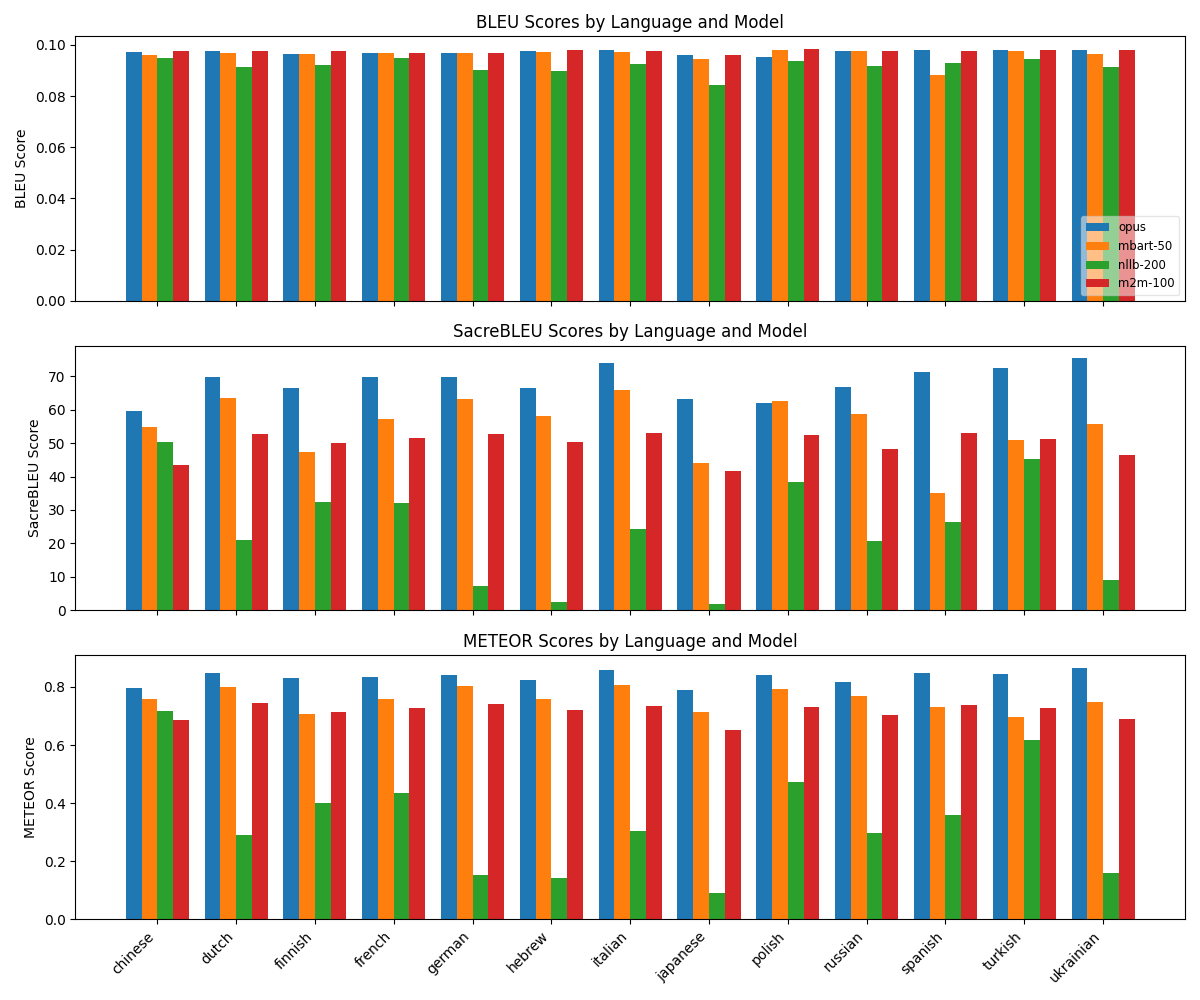
\includegraphics[width=1\linewidth]{figures/metrics_bar.png}
    \caption{BLEU, SacreBLEU, and METEOR scores of each model on each language.}
    \label{fig:result_visual}
\end{figure}

Figure \ref{fig:result_visual} shows the visualisation of all scores.

All models perform similarly on BLEU score across all languages, with NLLB-200 suffering a bit more on Japanese translation. The OPUS-MT model consistently shows high scores across most languages, with the highest SacreBLEU and METEOR scores overall, especially for Ukrainian and Italian. The mBART-50 model achieved the best-performing multilingual model, showing competitive performance, often achieving the second-highest scores across several languages. M2M-100 performs worse in SacreBLEU compared to mBART-50, but comparably similar in METEOR scores. The NLLB-200 model shows significant variability, especially for Japanese, where the SacreBLEU and METEOR scores are extremely low.

Dutch and Italian translations generally score higher across all metrics, suggesting that these languages are well-supported by the pre-trained models. Japanese translations, however, pose significant challenges for all models, as indicated by the consistently low scores across all metrics.

\begin{figure}[htbp]
    \centering
    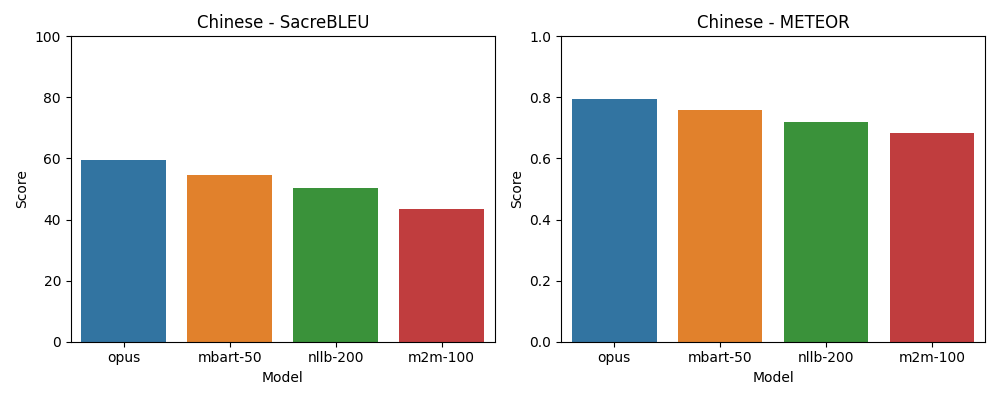
\includegraphics[width=0.49\linewidth]{figures/chinese_all_metrics.png}
    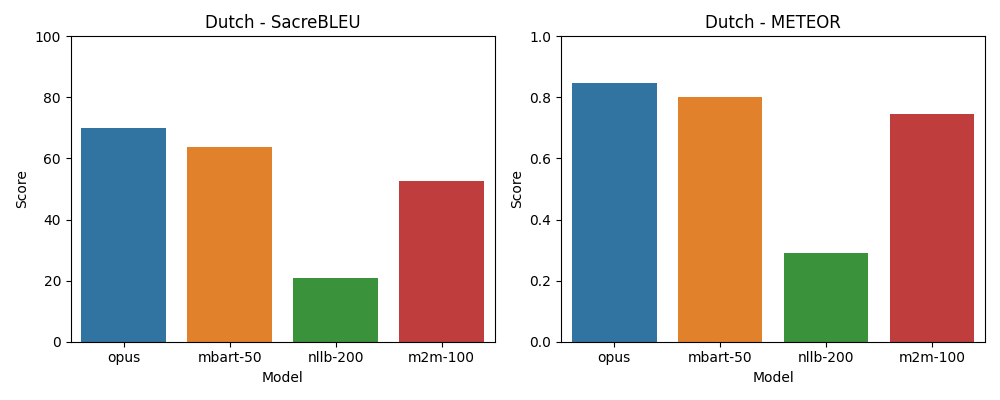
\includegraphics[width=0.49\linewidth]{figures/dutch_all_metrics.png}
    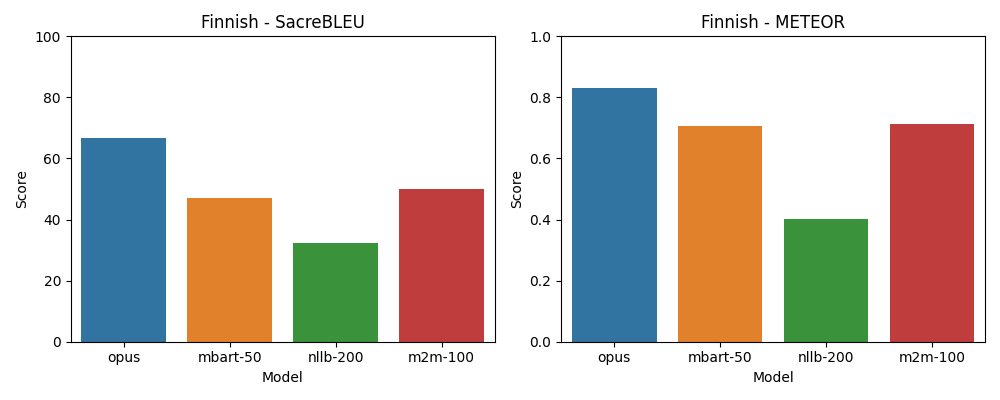
\includegraphics[width=0.49\linewidth]{figures/finnish_all_metrics.png}
    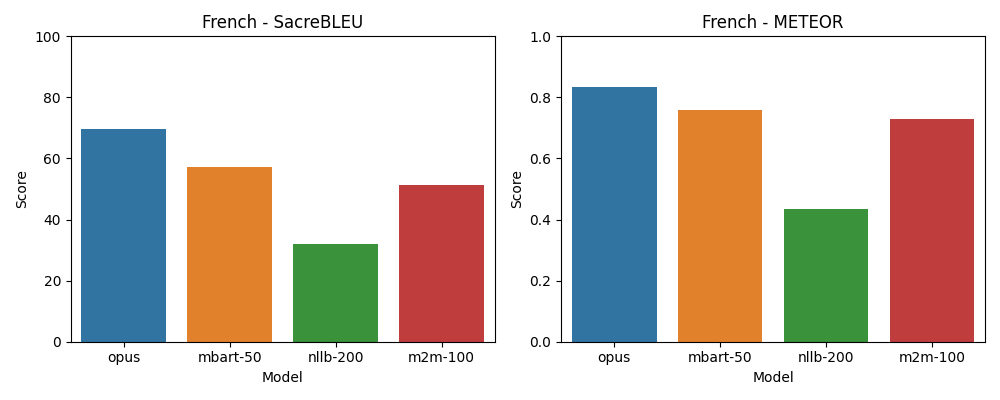
\includegraphics[width=0.49\linewidth]{figures/french_all_metrics.png}
    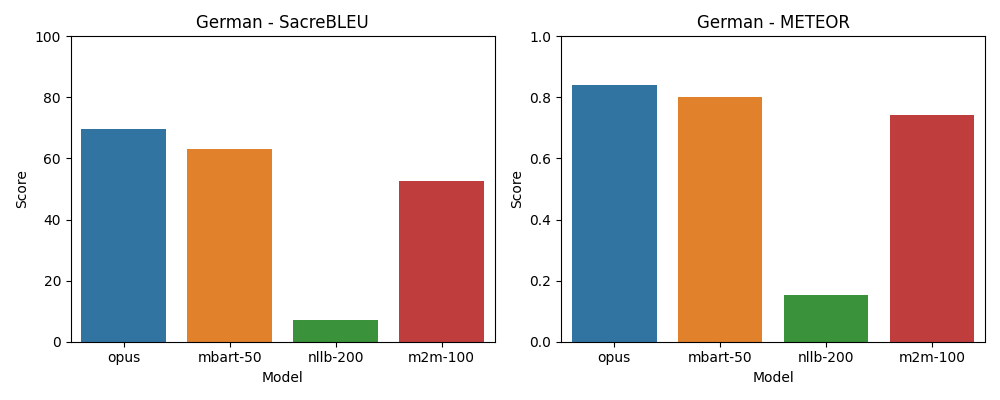
\includegraphics[width=0.49\linewidth]{figures/german_all_metrics.png}
    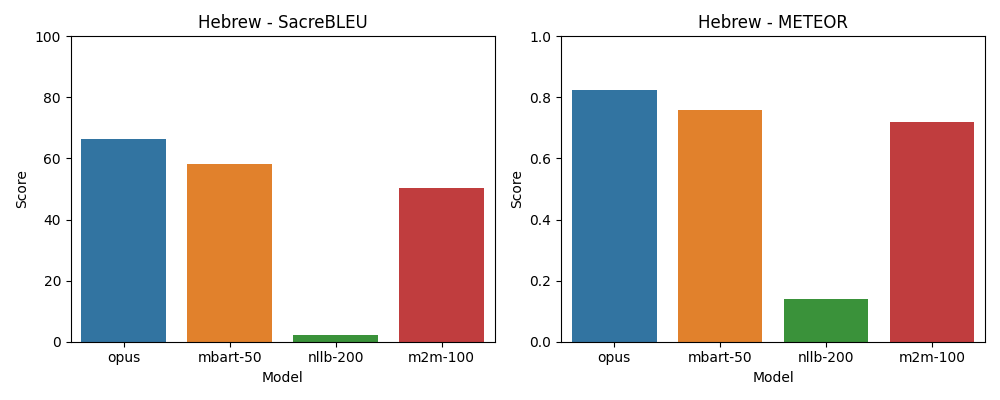
\includegraphics[width=0.49\linewidth]{figures/hebrew_all_metrics.png}
    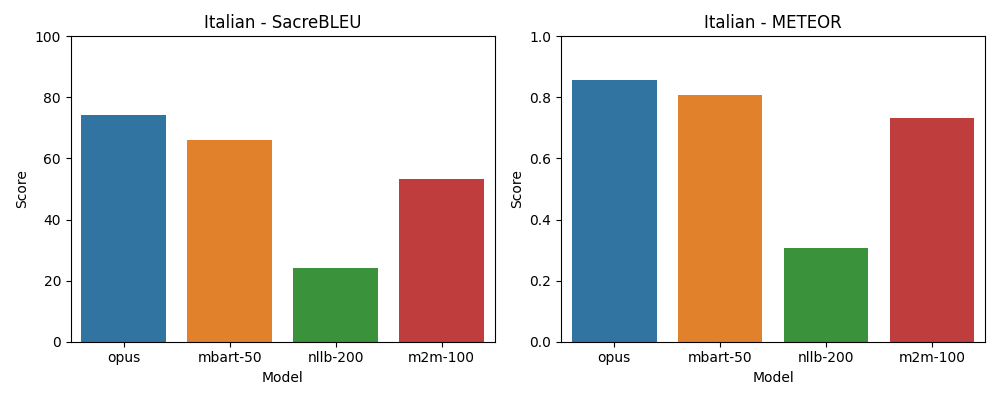
\includegraphics[width=0.49\linewidth]{figures/italian_all_metrics.png}
    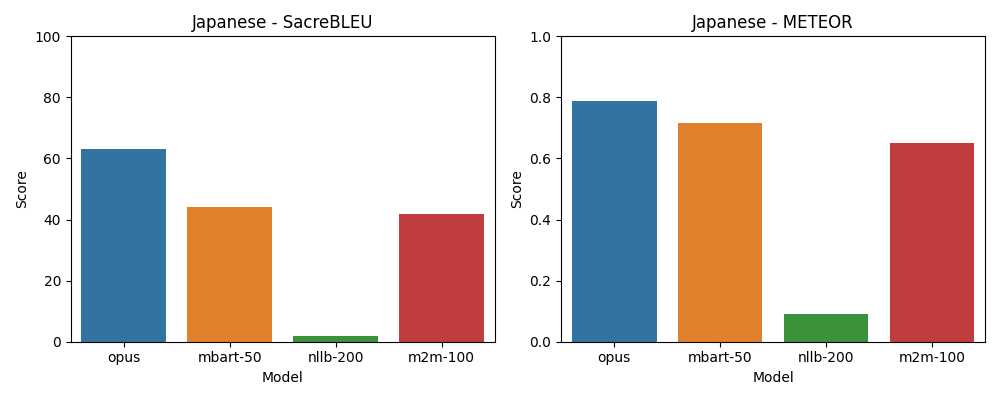
\includegraphics[width=0.49\linewidth]{figures/japanese_all_metrics.png}
    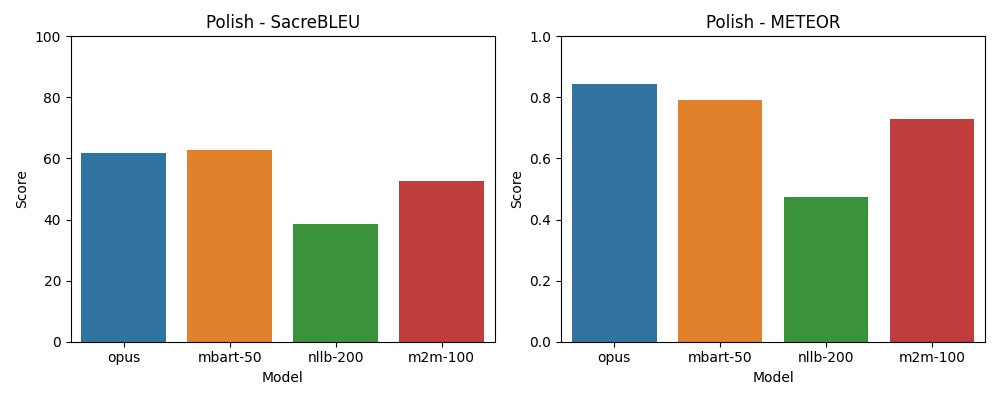
\includegraphics[width=0.49\linewidth]{figures/polish_all_metrics.png}
    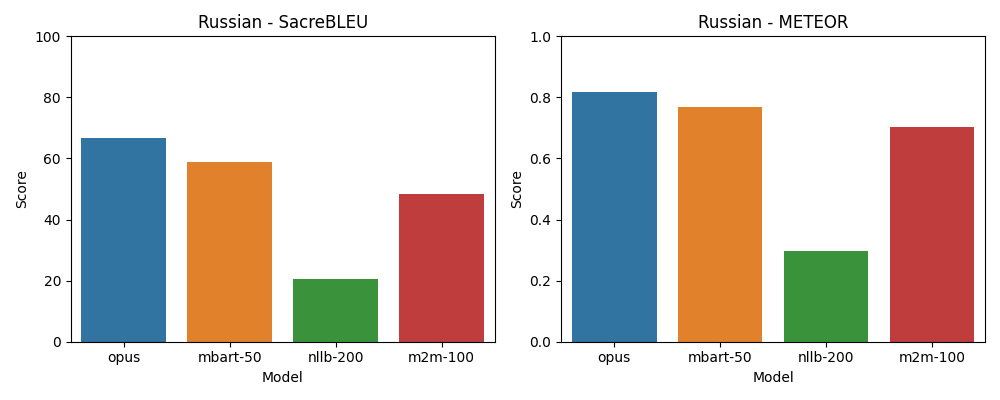
\includegraphics[width=0.49\linewidth]{figures/russian_all_metrics.png}
    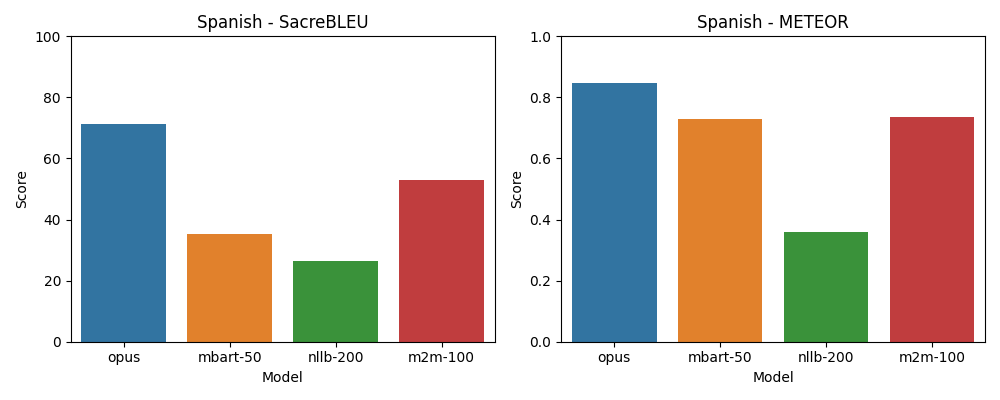
\includegraphics[width=0.49\linewidth]{figures/spanish_all_metrics.png}
    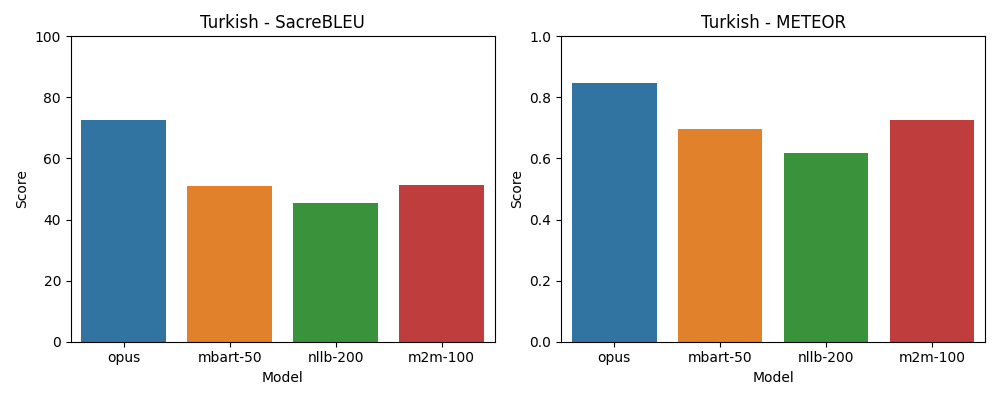
\includegraphics[width=0.49\linewidth]{figures/turkish_all_metrics.png}
    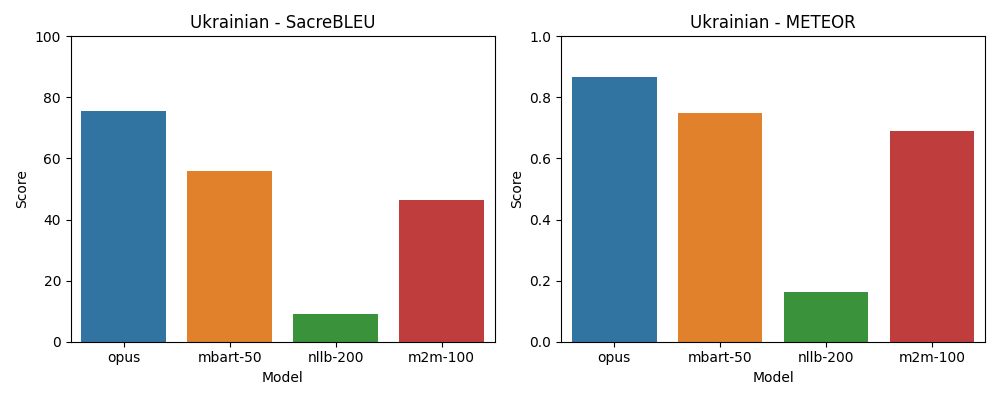
\includegraphics[width=0.49\linewidth]{figures/ukrainian_all_metrics.png}
    \caption{Performance of every language.}
    \label{fig:lang_metrics}
\end{figure}

Figure \ref{fig:lang_metrics} shows the SacreBLEU and METEOR scores for each language by model. The OPUS-MT and mBART-50 models are the clear winners in almost all languages. Although M2M-100 performs competitively with mBART-50 in most languages, it surpasses mBART-50 in Spanish-to-English translation. On the other hand, NLLB-200 performs the weakest, with extremely low scores in German, Hebrew, and Japanese.

\begin{figure}[htbp]
    \centering
    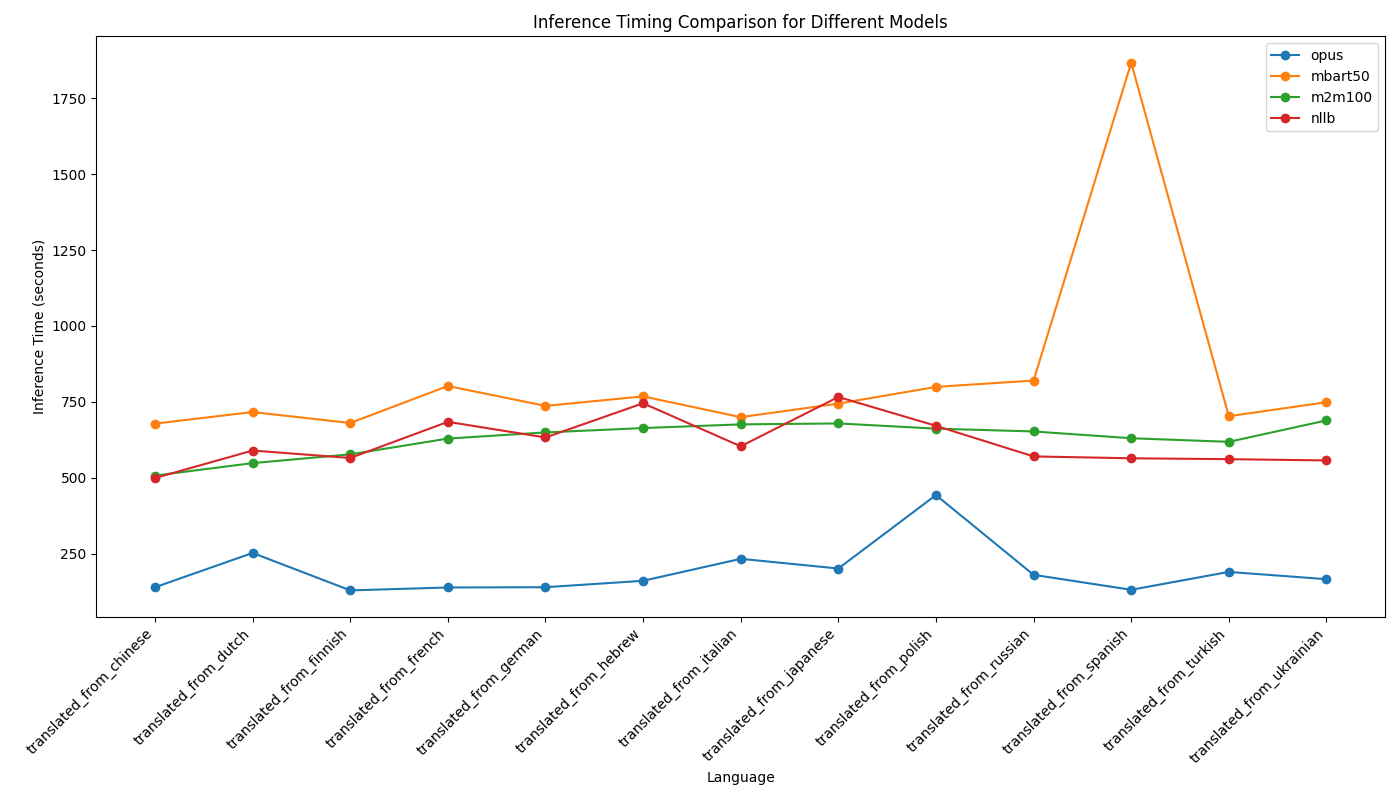
\includegraphics[width=0.9\linewidth]{figures/inference_timings.png}
    \caption{Inference timings for every model.}
    \label{fig:inference_timings}
\end{figure}

Figure \ref{fig:inference_timings} shows the time taken to translate for each language across experimented models. The OPUS-MT model is the fastest among the other three multilingual models, which perform similarly in timings. It is quite unclear why mBART50 Spanish-to-English translation suffers from a significantly higher timing. Re-running the experiment shows that this timing is consistent and not an anomaly.

\section{Conclusion}

This study findings show that while multilingual models have been shown to achieve higher performance compared to one-to-one translation models \cite{liu-2020-mbart}, this does not hold on short sentences, many-to-English translations across the 14 source languages. Additionally, mBART50 performed better than PTMs M2M-100 and NLLB-200 in these 14 languages.

Limitations, only the first translation of the same phrases are taken.
No fine-tuning is applied, which may affect the translation results, as fine-tuning models for specific languages can significantly improve models performance \cite{zhang-2023-fine-tuning}.

\section{Future Works}

Future works should be done by incorporating more Pre-Trained Models (PTMs) and incorporating fine-tuning for specific languages on languages-to-English translation. Evaluating with bigger datasets and longer texts can also be beneficial, as well as using language other than English as the target language.

Furthermore, it may be beneficial to consider more general multilingual PTMs such as mBERT \cite{wu-2020-mbert-are-all} and PolyLM \cite{wei-2023-polylm}, which are trained for a wide arrange of NLP tasks instead of just machine translation.

\printbibliography
\end{document}
